%%%%%%%%%%%%%%%%%%%%%%%%%%%%%%%%%%%%%%%%%
% fphw Assignment
% LaTeX Template
% Version 1.0 (27/04/2019)
%
% This template originates from:
% https://www.LaTeXTemplates.com
%
% Authors:
% Class by Felipe Portales-Oliva (f.portales.oliva@gmail.com) with template
% content and modifications by Vel (vel@LaTeXTemplates.com)
%
% Template (this file) License:
% CC BY-NC-SA 3.0 (http://creativecommons.org/licenses/by-nc-sa/3.0/)
%
%%%%%%%%%%%%%%%%%%%%%%%%%%%%%%%%%%%%%%%%%

%----------------------------------------------------------------------------------------
%	PACKAGES AND OTHER DOCUMENT CONFIGURATIONS
%----------------------------------------------------------------------------------------

\documentclass[
    12pt, % Default font size, values between 10pt-12pt are allowed
%letterpaper, % Uncomment for US letter paper size
%spanish, % Uncomment for Spanish
]{../fphw}

% Template-specific packages
\usepackage[utf8]{inputenc} % Required for inputting international characters
\usepackage[T1]{fontenc} % Output font encoding for international characters
\usepackage{mathpazo} % Use the Palatino font

\usepackage{graphicx} % Required for including images

\usepackage{booktabs} % Required for better horizontal rules in tables

\usepackage{listings} % Required for insertion of code

\usepackage{enumerate} % To modify the enumerate environment
\usepackage{enumitem}
\usepackage{textcomp}
\usepackage{amsmath}
\usepackage{subcaption}
\usepackage[justification=centering]{caption}
\usepackage{float}
\usepackage{xcolor}
\usepackage{polski}
\usepackage[polish]{babel}
\usepackage{csvsimple}
\usepackage{mathtools}
\usepackage{ulem}
\usepackage{hyperref}
\usepackage{makecell}
\usepackage{multirow}
\renewcommand{\cellalign}{cl}
\usepackage[ddmmyyyy]{datetime}
\renewcommand{\dateseparator}{.}

\definecolor{codegreen}{rgb}{0,0.6,0}
\definecolor{codegray}{rgb}{0.5,0.5,0.5}
\definecolor{codepurple}{rgb}{0.58,0,0.82}
\definecolor{backcolour}{rgb}{0.95,0.95,0.92}

\lstdefinestyle{mystyle}{
    backgroundcolor=\color{backcolour},
    commentstyle=\color{codegreen},
    keywordstyle=\color{magenta},
    numberstyle=\tiny\color{codegray},
    stringstyle=\color{codepurple},
    basicstyle=\ttfamily\footnotesize,
    breakatwhitespace=false,
    breakatwhitespace=false,
    breaklines=true,
    captionpos=b,
    keepspaces=true,
    numbers=left,
    numbersep=5pt,
    showspaces=false,
    showstringspaces=false,
    showtabs=false,
    tabsize=2
}

\lstset{style=mystyle}

\renewcommand{\lstlistlistingname}{Spis listingów}
%----------------------------------------------------------------------------------------
%	ASSIGNMENT INFORMATION
%----------------------------------------------------------------------------------------

\title{Projekt 2} % Assignment title

\author{inż.Monika Nawój} % Student name

\date{\today} % Due date

\institute{Politechnika Warszawska \\ Wydział Elektroniki i Technik Informacyjnych} % Institute or school name

\class{Zarządzanie i harmonogramowanie procesów} % Course or class name

\professor{mgr inż. Przemysław Kacprzak} % Professor or teacher in charge of the assignment

%----------------------------------------------------------------------------------------

\begin{document}

\maketitle % Output the assignment title, created automatically using the information in the custom commands above

%----------------------------------------------------------------------------------------
%	ASSIGNMENT CONTENT
%----------------------------------------------------------------------------------------

\section{Treść projektu}
Celem ćwiczenia jest zapoznanie z zagadnieniami produkcji
z mechanizmami aukcyjnymi.
Wskazówka: W przypadku jednego (a w zasadzie dwóch) zadań nie warto
wykorzystywać AMPLa.
\subsection {Szeregowanie zadań na jednakowych procesorach równoległych}
\subsubsection{Zadania podzielne}
Na podstawie podanych danych \(n\) - liczba procesów,
\(p_j\) - czas wykonania \(j\)-tego zadania, określić minimalny czas,
w jakim można zakończyć wszystkie zadania (\(C_{max}\)).
Stworzyć harmonogram realizujący wyznaczony czas.
\subsubsection{Zadania niepodzielne}
\begin{enumerate}[label=(\alph*)]
    \item \label{12a} Mając dane: \(n\) - liczba procesów, \(p_j\) - czas wykonania
          \(j\)-tego zadania, stworzyć model minimalizujący czas wykonania
          wszystkich zadań (\(C_{max}\)). Porównać wynik z rozwiązaniem,
          gdy zadania były podzielne.
          Jaka zależność zachodzi w ogólnym przypadku między rozwiązaniami tych zadań?
    \item \label{12b} Zaproponować regułę przydziału zadań minimalizującą czas
          wykonania wszystkich zadań (\(C_{max}\)).
          Porównać wynik z rozwiązaniem optymalnym - jaka zależność zachodzi w ogólnym przypadku?
    \item \label{12c} Mamy Rozwiązanie - niekoniecznie optymalne. Zaproponuj algorytm lokalnej poprawy rozwiązania.
\end{enumerate}

\subsection{Szeregowanie zadań na niejednorodowych procesorach równoległych}
\subsubsection{Zadania podzielne}
Mając dane \(p_{ij}\) — czas wykonania \(j\)-tego zadania na \(i\)-tym procesorze,
zaproponuj model minimalizujący czas wykonania wszystkich zadań (\(C_{max}\)).
\subsubsection{Zadania niepodzielne}
\begin{enumerate}[label=(\alph*)]
    \item \label{22a} Mając dane \(p_{ij}\) — czas wykonania j-tego zadania na i-tym procesorze,
          zaproponuj model minimalizujący czas wykonania wszystkich
          zadań (\(C_{max}\)).
    \item \label{22b} Mając dane \(p_{ij}\) — czas wykonania j-tego zadania na i-tym procesorze,
          zaproponuj model minimalizujący sumę czasów przebywania w
          systemie (\(\sum F_j\))
    \item \label{22c} czas wykonania j-tego zadania na i-tym procesorze,
          zaproponuj model minimalizujący sumę czasów oczekiwania na obsługę.
          (Wskazówka - czym różni ten punkt od poprzedniego)
\end{enumerate}

\subsection{Modernizacja oświetlenia}
W związku ze wzrostem cen energii elektrycznej oraz zmianami cen źródeł światła wspólnota mieszkaniowa rozważa modernizację oświetlenia.
Rozważana jest modernizacja oświetlenia wejść do 3 klatek schodowych, w każdym wejściu
mamy po dwie oprawy świetlówkowe 36W (rzeczywisty pobór mocy 44 W),
obecnie do włączania wykorzystywana jest fotokomórka. Można oszacować
że w roku włączane jest raz dziennie, a średni czas włączenia do 10h/dzień, w
przypadku dodatkowego zastosowania czujników ruchu można się spodziewać
średnio 150 włączeń/dzień, średni czas włączenia to 1,5 min.

W istniejących oprawach świetlówkowych zostały zastosowane stateczniki elektromagnetyczne. Koszt wymiany przepalonych świetlówek z jednej
oprawy to 10zł. Modernizacja może obejmować instalację czujników ruchu
– jednorazowy wydatek 200zł na oprawę oraz modernizację źródeł światła,
która może obejmować:
\begin{itemize}
    \item wymianę stateczników elektromagnetycznych na elektroniczne z ciepłym startem
          – jednorazowy wydatek 140zł/szt., przy czym obniża się moc pojedynczej oprawy do 40W,
    \item wymianę na oświetlenie LED, koszt zmiany to 200 zł, koszt wymiany
          to 180 zł, skutkiem jest zmniejszenie mocy oprawy do 25W.
\end{itemize}
Wszystkie podane ceny to ceny brutto, WM płaci za energię elektryczną według taryfy G11.

\textbf{Trwałość źrodeł światła}
Trwałość wszystkich źródeł światła jest modelowana
w ten sam sposób – przeciętnie źródło światła trzeba wymienić, gdy
wyrażenie \(\frac{H}{L_h} + \frac{S}{L_s}\)
osiągnie wartość \(1\), gdzie \(H\) to liczba godzin pracy źródła,
a \(S\) to liczba włączeń, parametry \(L_h\) i \(L_s\) można odczytać z tabeli poniżej.
\begin{table}[H]
    \centering
    \begin{tabular}{| c | c | c |}
        \hline
        Typ                          & \(L_h\) [h] & \(L_s\)       \\
        \hline
        świetlówka stat. elektromag. & 16 000      & 8 000         \\
        świetlówka ciepły start      & 16 000      & 50 000        \\
        Halogen                      & 3 000       & \( \infty  \) \\
        LED                          & 50 000      & \( \infty  \) \\
        \hline
    \end{tabular}
    \caption{Trwałość wszystkich źródeł światła}
\end{table}

\textbf{Zadanie} Wybierz miarę według której zostanie wybrany najlepszy wariant,
określ długosc horyzontu (podaj uzasadnienie) i wybierz najlepszy wariant.
Jako stopę dyskonta wybierz 10\%. Co się stanie, jeżeli będzie to 5\% lub 15\%.

\subsection{Planowanie produkcji realizowanej w porcjach}
W tym zadaniu celem jest zaplanowanie produkcji. Dane jest zapotrzebowanie na produkty końcowe,
które należy zaspokoić pod koniec określonych okresów czasu. Do wytworzenia poszczególnych produktów potrzebne
są pewne półprodukty. Produkcja poszczególnych produktów trwa określony czas.
Produkcja charakteryzuje się stałym kosztem, który trzeba ponięść,
jeżeli w danym okresie inicjujemy produkcję, tzn. w tym etapie są pobierane
półprodukty potrzebne do produkcji, dana partia będzie dostępna po okresie
równym czasowi produkcji. Wszystkie produkty mogą być magazynowane,
przy czym magazynowanie kosztuje.
Należy określić, ile i kiedy, jakich wyrobów (równiez półproduktów) produkować.

\begin{enumerate}
    \item stwórz i rozwiąż model, opisujący warstwę wyrobów finalnych (koszty
          wytworzenia półproduktów pomijamy)
    \item stwórz i rozwiąż dokładny model (zadanie programowani liniowego mie-
          szanego) opisujący całe zadanie.
\end{enumerate}

\subsection{Aukcje}
Na aukcji zostało wystawionych n jednakowych przedmiotów. Oferty uczestników zostaną podane razem z pozostałymi danymi.

\begin{enumerate}
    \item \label{51} wyznacz rozwiązanie aukcji niejawnej pierwszej ceny,
    \item \label{52} wyznacz rozwiązania aukcji Vicrey`a,
    \item \label{53} wyznacz rozwiązanie niejawnej aukcji jednolitej ceny (ceny pierwszej
          odrzuconej oferty)
    \item \label{54} wyznacz rozwiązanie aukcji niejawnej pierwszej ceny,
          jesli wystawiający mogą poznać złożone oferty i zmniejszyć liczbę wystawianych
          przedmiotów, w celu zwiększenia przychodu,
    \item \label{55} wyznacz rozwiązania aukcji Vicrey’a, jesli wystawiający może poznać
          złożone oferty i zmniejszyć liczbę wystawianych przedmiotów, w celu
          zwiększenia przychodu,
    \item \label{56} wyznacz rozwiązanie niejawnej aukcji jednolitej ceny (ceny pierwszej
          odrzuconej oferty), jesli wystawiający może poznać złożone oferty i
          zmniejszyć liczbę wystawianych przedmiotów, w celu zwiększenia przychodu
\end{enumerate}
\newpage
\section{Dane}
\subsection{Procesy jednakowe}
\begin{itemize}
    \item liczba procesów \(n = 2\)
\end{itemize}
\begin{table}[H]
    \centering
    \begin{tabular}{| c | c |}
        \hline
        Zadanie & Czas obsługi \(p_j\) \\
        \hline
        A       & 16                   \\
        B       & 12                   \\
        C       & 5                    \\
        D       & 12                   \\
        E       & 14                   \\
        F       & 6                    \\
        G       & 8                    \\
        H       & 7                    \\
        \hline
    \end{tabular}
    \caption{Czas wykonywania zadań}
\end{table}

\subsection{Procesy różne}
\begin{table}[H]
    \centering
    \begin{tabular}{| c | c | c |}
        \hline
        Zadanie & Czas obsługi na 1. procesorze - \(p_{1j}\) & Czas obsługi na 2. procesorze - \(p_{2j}\) \\
        \hline
        A       & 14                                         & 9                                          \\
        B       & 14                                         & 16                                         \\
        C       & 5                                          & 7                                          \\
        D       & 11                                         & 9                                          \\
        E       & 14                                         & 12                                         \\
        F       & 12                                         & 16                                         \\
        G       & 8                                          & 4                                          \\
        H       & 9                                          & 17                                         \\
        \hline
    \end{tabular}
    \caption{Czas obsługi na poszczególnych procesorach}
\end{table}

\subsection{Planowanie produkcji realizowanej w porcjach}
\begin{table}[H]
    \centering
    \begin{tabular}{| c | c | c | c | c | c | c | c | c |}
        \hline
                            & A  & B  & C  & D & E & F & G  & H \\
        \hline
        Czas produkcji      & 1  & 2  & 1  & 1 & 3 & 1 & 1  & 2 \\
        Koszt uruch. prod.  & 20 & 12 & 15 & 7 & 5 & 2 & 19 & 9 \\
        Koszt magazynowania & 4  & 2  & 2  & 1 & 1 & 1 & 1  & 2 \\
        \hline
    \end{tabular}
    \caption{Czas obsługi na poszczególnych procesorach}
\end{table}

\begin{table}[H]
    \centering
    \begin{tabular}{| c | c | c | c | c | c | c | c | c | c |}
        \hline
                & 1 & 2 & 3 & 4 & 5 & 6 & 7 & 8  & 9  \\
        \hline
        Wyrób A &   &   &   &   &   & 4 & 5 & 8  & 16 \\
        \hline
        Wyrób B &   &   &   &   &   &   & 9 & 18 & 23 \\
        \hline
        Wyrób C &   &   &   &   &   &   & 5 & 17 & 22 \\
        \hline
    \end{tabular}
    \caption{Zapotrzebowanie na wyroby finalne(na koniec poszczególnych okresów)}
\end{table}

\begin{figure}[H]
    \centering
    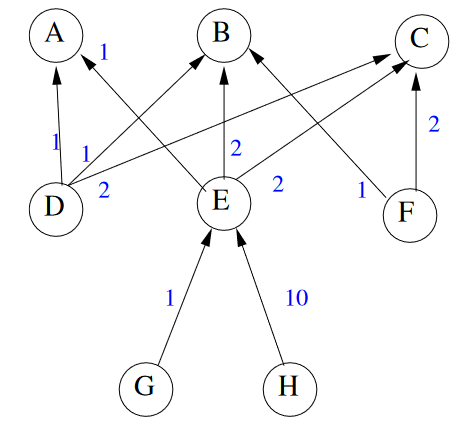
\includegraphics[width=0.7\linewidth]{./img/zaleznosci.PNG}
    \caption{Zależności między towaram}
    \label{fig:graf-1}
\end{figure}

Rysunek ~\ref{fig:graf-1} przedstawia zależności między towarami
(np. do wytworzenia jednej sztuki wyrobu E potrzeba 1 sztuki wyrobu G i 10 sztuk wyrobu H).

\subsection{Aukcje}
Liczba przedmiotów \(n = 3\) \\
\begin{table}[H]
    \centering
    \begin{tabular}{| c | c |}
        \hline
        Uczestnik & Kolejne ceny \\
        \hline
        A         & 25, 8, 3     \\
        B         & 18, 7, 4     \\
        C         & 20, 2, 5     \\
        \hline
    \end{tabular}
    \caption{Oferty}
\end{table}

\newpage
\section{Rozwiązanie}
\subsection{Szeregowanie zadań na jednakowych procesorach równoległych}
Dane do zadania zostały zapisane w języku AMPL.
\lstinputlisting[caption=Dane w języku AMPL]{./src/dane-1.dat}
Dane zostały załączone w pliku \textit{dane-1.dat}.
\subsubsection{Zadania podzielne}
Problem przestawiony w niniejszym zadaniu jest problemem \(P|pmtn|C_{max}\)
tj. problem szeregowania podzielnych i niezależnych zadań na dwóch procesorach z kryterium \(C_{max}\). \\
Model matematyczny przedstawia się następująco: \\ \\
Parametry modelu: \\
\(x_{ij}\) - czas przetwarzania na procesorze \(i\) zadania \(j\) \\
\(p_j\) - czas przetwarzania zadania \(j\) \\ \\
Zmienne decyzyjne: \\
\(C_{max}\) - zmienna określająca maksymalny czas przetwarzania zadań na obu procesorach \\ \\
Funkcja celu: \\
\begin{align*}
    min \text{ } C_{max}
\end{align*}
Przy ograniczeniach: \\
\begin{align*}
     & \sum^m_{j=1}x_{ij} = p_j \leq C_{max} \\
     & \sum^n_{i=1}x_{ij} \leq C_{max}       \\
     & \sum^m_{j=1}x_{ij} \leq C_{max}       \\
     & x_{ij} \geq 0
\end{align*}
gdzie:
\begin{align*}
     & j = 1, ..., m; \\
     & i = 1, ..., n;
\end{align*}

\lstinputlisting[caption=Model w języku AMPL]{./src/model-1.mod}
Model został załączony w pliku \textit{model-1.mod}.


\begin{lstlisting}[caption=Rozwiązanie znalezione solwerem minos]
    MINOS 5.51: optimal solution found.
    4 iterations, objective 40
    x :=
    1 A    0
    1 B    0
    1 C    0
    1 D    5
    1 E   14
    1 F    6
    1 G    8
    1 H    7
    2 A   16
    2 B   12
    2 C    5
    2 D    7
    2 E    0
    2 F    0
    2 G    0
    2 H    0
    ;
    == 1 ==========================
\end{lstlisting}
Zgodnie z wynikami wyznaczonymi przez solver MINOS wartość \(C_{max}\) wynosi 40 jednostek czasu.
Jedynym podzielonym zadaniem jest \textbf{zadanie D}: 5 jednostek czasu zostaje obsłużone na \textit{procesorze 1}
oraz 7 jednostek czasu zostaje obsłużone na \textit{procesorze 2}.
Dla ułatwienia przedstawiam dodatkowo rozwiązanie w formie tabeli.
\begin{table}[H]
    \centering
    \begin{tabular}{| c | c | c | c | c | c | c | c | c |}
        \hline
        Zadanie    & A  & B  & C & D & E  & F & G & H \\
        \hline
        Procesor 1 &    &    &   & 5 & 14 & 6 & 8 & 7 \\
        \hline
        Procesor 2 & 16 & 12 & 7 & 7 &    &   &   &   \\
        \hline
    \end{tabular}
    \caption{Czas przetwarzania poszczególnych zadań na wybranych procesorach}
\end{table}


\begin{figure}[H]
    \centering
    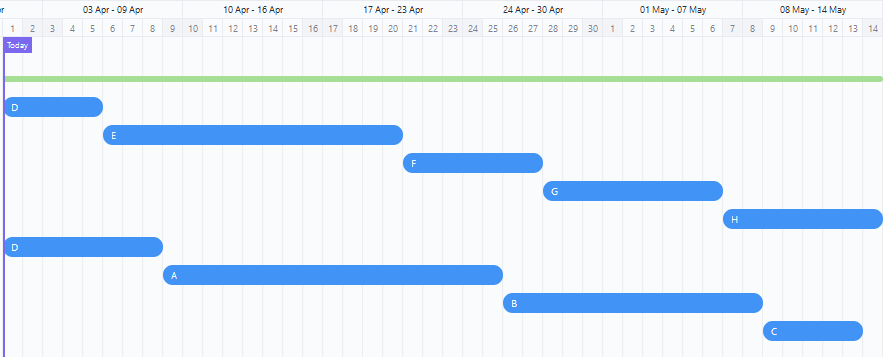
\includegraphics[width=\linewidth]{./img/harmonogram-1.PNG}
    \caption{Harmonogram realizujący wyznaczony czas}
    \label{fig:harmonogram-1}
\end{figure}

Rysunek ~\ref{fig:harmonogram-1} przedstawia harmonogram wyznaczonego czasu
w formie wykresu Gantta, gdzie jedna jednostka czasu jest równa jednemu dniowi.

\subsubsection{Zadania niepodzielne}
\par\noindent\rule{\textwidth}{0.4pt}
Podpunkt \ref{12a}
\par\noindent\rule{\textwidth}{0.4pt}
W przypadku zadania niepodzielnego jest to problem \(P||C_{max}\)
tj. problem zadań niepodzielnych na dwóch procesorach z kryterium \(C_{max}\). \\
Model przedstawia się następująco: \\ \\
Parametry modelu: \\
\(x_{ij}\) - czas przetwarzania na procesorze \(i\) zadania \(j\) \\
\(p_j\) - czas przetwarzania zadania \(j\) \\ \\
Zmienne decyzyjne: \\
\(C_{max}\) - zmienna określająca maksymalny czas przetwarzania zadań na obu procesorach \\ \\
Funkcja celu: \\
\begin{align*}
    min \text{ } C_{max}
\end{align*}
\newpage
Przy ograniczeniach: \\
\begin{align*}
     & \sum^m_{i=1}x_{ij} \cdot p_j \leq C_{max} \\
     & \sum^n_{j=1}x_{ij} = 1                    \\
     & x \in  {0,1}
\end{align*}
gdzie:
\begin{align*}
     & j = 1, ..., m; \\
     & i = 1, ..., n;
\end{align*}

\lstinputlisting[caption=Model w języku AMPL]{./src/model-2.mod}
Model został załączony w pliku \textit{model-2.mod}.

\begin{lstlisting}[caption=Rozwiązanie znalezione solwerem lpsolve]
    LP_SOLVE 4.0.1.0: optimal, objective 40
    161 simplex iterations
    129 branch & bound nodes: depth 9
    x :=
    1 A   0
    1 B   0
    1 C   1
    1 D   0
    1 E   1
    1 F   1
    1 G   1
    1 H   1
    2 A   1
    2 B   1
    2 C   0
    2 D   1
    2 E   0
    2 F   0
    2 G   0
    2 H   0
    ;
    == 1 ==========================
\end{lstlisting}
Zgodnie z wynikami wyznaczonymi przez solver lpsolve wartość \(C_{max}\) nadal wynosi 40 jednostek czasu
nawet przy niepodzielności zadań.

\newpage

Dla ułatwienia przedstawiam dodatkowo rozwiązanie w formie tabeli.
\begin{table}[H]
    \centering
    \begin{tabular}{| c | c | c | c | c | c | c | c | c |}
        \hline
        Zadanie    & A  & B  & C & D  & E  & F & G & H \\
        \hline
        Procesor 1 &    &    & 7 &    & 14 & 6 & 8 & 7 \\
        \hline
        Procesor 2 & 16 & 12 &   & 12 &    &   &   &   \\
        \hline
    \end{tabular}
    \caption{Czas przetwarzania poszczególnych zadań na wybranych procesorach}
\end{table}

Porównując rozwiązanie zadania podzielnego i nie podzielnego,
oczywistą różnicą jest przydzielenie \textbf{zadania D} do tylko jednego procesora,
którym jest \textit{procesor 2},
Kolejną różnicą jest przetworzenie \textbf{zadania C} w wariancie podzielnym
na \textit{procesorze 2}, natomiast w wariancie niepodzielnym na \textit{procesorze 1}.
Całkowity czas przetwarzania wszystkich zadań jest niezmienny niezależnie od wariantu.
\par\noindent\rule{\textwidth}{0.4pt}
Podpunkt \ref{12b}
\par\noindent\rule{\textwidth}{0.4pt}
Proponowaną regułą przydziału zadań minimalizującą czas wykonywania wszystkich
zadań \(C_{max}\) jest szeregowanie listowe przy użyciu zasady LPT (ang. \textit{Longest Processing Time}).
Metoda ta pozwala wybór kolejności zadań według ustalonej listy priorytetów.
Po zakończeniu przetwarzania pierwszych zadań i zwolnieniu zasobów
procesorów, przydzielane jest kolejne zadanie z listy do procesora,
który gwarantuje najwcześniejszy czas ukończenia zadania.

\par\noindent\rule{\textwidth}{0.4pt}
Podpunkt \ref{12c}
\par\noindent\rule{\textwidth}{0.4pt}
W przypadku zadania niekoniecznie optymalnego w przypadku problemu \(P||C_{max}\)
należy wykorzystać metodę \textbf{LPT} zgodnie z wykładem:
\begin{quote}
    W przypadku Problemu \(P ||C_{max}\) najlepszy wartiant algorytmu szeregowania listowego LS wykorzystuje regułę priorytetową LPT.
    Wtedy długość uszeregowania \(C_{max}\) jest w najgorszym przypadku nie gorsza od optymalnej wartości \(C_{max}\)
    co najwyżej \( (\frac{4}{3} - \frac{1}{3m} )\) razy.
\end{quote}
\newpage
\subsection{Szeregowanie zadań na niejednorodowych procesorach równoległych}
Dane do zadania zostały zapisane w języku AMPL.
\lstinputlisting[caption=Dane w języku AMPL]{./src/dane-2.dat}
Dane zostały załączone w pliku \textit{dane-2.dat}.
\subsubsection{Zadania podzielne}
Problemem przedstawionym w zadaniu jest problem \(R|pmtn|C_{max}\)
tj. problem szeregowania \(n\) zadań niezależnych i podzielnych
na \(m\) procesorach równoległych, gdzie:
\begin{align*}
     & n = 8 \\
     & m = 2
\end{align*}
Model matematyczny przedstawia się następująco: \\ \\
Parametry modelu: \\
\(x_{ij}\) - czas przetwarzania na procesorze \(i\) zadania \(j\) \\
\(p_{ji}\) - czas przetwarzania zadania \(j\) na procesorze \(i\) \\ \\
Zmienne decyzyjne: \\
\(C_{max}\) - zmienna określająca maksymalny czas przetwarzania zadań na obu procesorach \\ \\
Funkcja celu: \\
\begin{align*}
    min \text{ } C_{max}
\end{align*}
Przy ograniczeniach: \\
\begin{align*}
     & \sum^m_{i=1} \frac{x_{ij}}{p_j}  \\
     & \sum^n_{j=1} x_{ij} \leq C_{max} \\
     & \sum^m_{i=1} x_{ij} \leq C_{max} \\
\end{align*}
gdzie:
\begin{align*}
     & j = 1, ..., m; \\
     & i = 1, ..., n;
\end{align*}
\lstinputlisting[caption=Model w języku AMPL]{./src/model-3.mod}
Model został załączony w pliku \textit{model-3.mod}.

\newpage

\begin{lstlisting}[caption=Rozwiązanie znalezione solwerem lpsolve]
    LP_SOLVE 4.0.1.0: optimal, objective 37.2
    10 simplex iterations
    x :=
    1 A    0
    1 B   11.2
    1 C    5
    1 D    0
    1 E    0
    1 F   12
    1 G    0
    1 H    9
    2 A    9
    2 B    3.2
    2 C    0
    2 D    9
    2 E   12
    2 F    0
    2 G    4
    2 H    0
    ;
    == 1 ==========================
\end{lstlisting}
Solwer lpsolve wyznaczył wartość \(C_{max}\) wynoszącą \(37.2\) jednostki czasu.
Warto zauważyć, że jedynym podzielonym zadaniem jest \textbf{zadanie B},
pozostałe zadania zostały wykonane w całości na jednym, wybranym procesorze.

Dla ułatwienia przedstawiam dodatkowo rozwiązanie w formie tabeli.
\begin{table}[H]
    \centering
    \begin{tabular}{| c | c | c | c | c | c | c | c | c |}
        \hline
        Zadanie    & A & B    & C & D & E  & F  & G & H \\
        \hline
        Procesor 1 &   & 11.2 & 5 &   &    & 12 &   & 9 \\
        \hline
        Procesor 2 & 9 & 3.2  &   & 9 & 12 &    & 4 &   \\
        \hline
    \end{tabular}
    \caption{Czas przetwarzania poszczególnych zadań na wybranych procesorach}
\end{table}

\newpage

\subsubsection{Zadania niepodzielne}
\par\noindent\rule{\textwidth}{0.4pt}
Podpunkt \ref{22a}
\par\noindent\rule{\textwidth}{0.4pt}
Przedstawiony w treści zadania problem jest problemem \(R||C_{max}\),
jego rozwiązanie możemy znaleźć poprzez rozwiązanie zadania programowania liniowego
ze zmiennymi binarnymi. \\
Model matematyczny przedstawia się następująco: \\ \\
Parametry modelu: \\
\(x_{ij}\) - czas przetwarzania na procesorze \(i\) zadania \(j\) \\
\(p_{ji}\) - czas przetwarzania zadania \(j\) na procesorze \(i\) \\ \\
Zmienne decyzyjne: \\
\(C_{max}\) - zmienna określająca maksymalny czas przetwarzania zadań na obu procesorach \\ \\
Funkcja celu: \\
\begin{align*}
    min \text{ } C_{max}
\end{align*}
Przy ograniczeniach: \\
\begin{align*}
     & \sum^m_{i=1} p_{ji} \cdot x_{ij} \leq C_{max} \\
     & \sum^n_{j=1} x_{ij} = 1                       \\
     & x_{ij} \in  \{0,1\}                           \\
\end{align*}
gdzie:
\begin{align*}
     & j = 1, ..., m; \\
     & i = 1, ..., n;
\end{align*}

\newpage
\lstinputlisting[caption=Model w języku AMPL]{./src/model-4.mod}
Model został załączony w pliku \textit{model-4.mod}.


\begin{lstlisting}[caption=Rozwiązanie znalezione solwerem lpsolve]
    LP_SOLVE 4.0.1.0: optimal, objective 40
    62 simplex iterations
    39 branch & bound nodes: depth 8
    x :=
    1 A   0
    1 B   0
    1 C   1
    1 D   0
    1 E   1
    1 F   1
    1 G   0
    1 H   1
    2 A   1
    2 B   1
    2 C   0
    2 D   1
    2 E   0
    2 F   0
    2 G   1
    2 H   0
    ;
    == 1 ==========================  
\end{lstlisting}

Zgodnie z wynikami wyznaczonymi przez solver lpsolve, czas maksymalny \(C_{max}\) wynosi 40 jednostek czasu,
czyli jest o \(2.8\) jednostek czasu dłuższy niż w przypadku wariantu z zadanimi podzielonymi.

Dla ułatwienia przedstawiam dodatkowo rozwiązanie w formie tabeli.
\begin{table}[H]
    \centering
    \begin{tabular}{| c | c | c | c | c | c | c | c | c |}
        \hline
        Zadanie    & A & B  & C & D & E  & F  & G & H \\
        \hline
        Procesor 1 &   &    & 5 &   & 12 & 12 &   & 9 \\
        \hline
        Procesor 2 & 9 & 14 &   & 9 &    &    & 4 &   \\
        \hline
    \end{tabular}
    \caption{Czas przetwarzania poszczególnych zadań na wybranych procesorach}
\end{table}

\newpage

\par\noindent\rule{\textwidth}{0.4pt}
Podpunkt \ref{22b}
\par\noindent\rule{\textwidth}{0.4pt}
W przedstawionym zadaniu minimalizujemy czas przetwarzania \textit{j-tego}
zadania na \textit{i-tym} procesorze.
Rozwiązanie tego problemu możemy znaleźć za pomocą reguły SPT (ang. \textit{Shortest Processing Time}).
Metoda ta pozwala na uszeregowanie zadań w kolejności rosnącego czasu przetwarzania zadania \(p_j\).
Wartość funkcji celu \(\sum F_j\) dla uzyskanego zbioru możemy zilutstrować jako pole pod wykresen.
Uszeregowane zadania wykonywane są w kolejności od najkrótszego do najdłuższego,
oznacza to iż cel minimalizacji czasu przetwarzania na procesorze zostaje osiagnięty.

Model matematyczny przedstawia się następująco: \\ \\
Parametry modelu: \\
\(p_{ji}\) - czas przetwarzania zadania \(j\) na procesorze \(i\) \\ \\
\(o_{k}\) - kolejność przetwarzania zadań \\ \\
Zmienne decyzyjne: \\
\(x_{ijk}\) - czas przetwarzania na procesorze \(i\) zadania \(j\) \\
\(C_{max}\) - zmienna określająca maksymalny czas przetwarzania zadań na obu procesorach \\ \\
Funkcja celu: \\
\begin{align*}
    min \sum^m_{i=1}\sum^n_{j=1}\sum^n_{k=1} k \cdot p_{ji} \cdot x_{ijk}
\end{align*}
Przy ograniczeniach: \\
\begin{align*}
     & \sum^m_{i=1} \sum^n_{j=1} x_{ijk} = 1 \\
     & \sum^n_{j=1} x_{ijk} \leq 1           \\
     & x_{ijk} \in  \{0,1\}                  \\
\end{align*}
\begin{align*}
     & j = 1, ..., m; \\
     & i = 1, ..., n;
     & k = 1, ..., n;
\end{align*}

\newpage

Dane do zadania zostały zapisane w języku AMPL.
\lstinputlisting[caption=Dane w języku AMPL]{./src/dane-3.dat}
Dane zostały załączone w pliku \textit{dane-3.dat}.

\lstinputlisting[caption=Model w języku AMPL]{./src/model-5.mod}
Model został załączony w pliku \textit{model-5.mod}.

\newpage

\begin{lstlisting}[caption=Rozwiązanie znalezione solwerem lpsolve]
    LP_SOLVE 4.0.1.0: optimal, objective 158
    21 simplex iterations
    x [1,*,*]
    :   1   2   3   4   5   6   7   8    :=
    A   0   0   0   0   0   0   0   0
    B   1   0   0   0   0   0   0   0
    C   0   0   0   1   0   0   0   0
    D   0   0   0   0   0   0   0   0
    E   0   0   0   0   0   0   0   0
    F   0   1   0   0   0   0   0   0
    G   0   0   0   0   0   0   0   0
    H   0   0   1   0   0   0   0   0
    
     [2,*,*]
    :   1   2   3   4   5   6   7   8    :=
    A   0   0   1   0   0   0   0   0
    B   0   0   0   0   0   0   0   0
    C   0   0   0   0   0   0   0   0
    D   0   1   0   0   0   0   0   0
    E   1   0   0   0   0   0   0   0
    F   0   0   0   0   0   0   0   0
    G   0   0   0   1   0   0   0   0
    H   0   0   0   0   0   0   0   0
    ;
    == 1 ==========================
\end{lstlisting}

Kolejność wykonywania zadań wyznaczona przez solver lpsolve
oznacza kolejność wykonywanych zadań od końca.
Poniżej przedstawiam interpretacje wyników w formie tabeli:

\begin{table}[H]
    \centering
    \begin{tabular}{| c | c | c | c | c | c | c | c | c |}
        \hline
        Zadanie    & 1 & 2 & 3 & 4 & 5 & 6 & 7 & 8 \\
        \hline
        Procesor 1 & C & H & F & B &   &   &   &   \\
        \hline
        Procesor 2 & G & A & D & E &   &   &   &   \\
        \hline
    \end{tabular}
    \caption{Kolejność przetwarzania poszczególnych zadań na wybranych procesorach}
\end{table}

\newpage

\par\noindent\rule{\textwidth}{0.4pt}
Podpunkt \ref{22c}
\par\noindent\rule{\textwidth}{0.4pt}
W opisanym przypadku celem jest minimalizacja czasu oczekiwania na przetworzenie zadania.
Model matematyczny jest analogiczny do tego z podpunktu \ref{22b},
z drobną modyfikacją funkcji celu, gdzie zamieniamy \(k\) na \((k-1)\).

\lstinputlisting[caption=Model w języku AMPL]{./src/model-6.mod}
Model został załączony w pliku \textit{model-6.mod}.

\begin{lstlisting}[caption=Rozwiązanie znalezione solwerem lpsolve]
    LP_SOLVE 4.0.1.0: optimal, objective 84
    26 simplex iterations
    x [1,*,*]
    :   1   2   3   4   5   6   7   8    :=
    A   0   0   0   0   0   0   0   0
    B   0   0   0   0   0   0   0   0
    C   0   0   0   1   0   0   0   0
    D   0   0   0   0   0   0   0   0
    E   1   0   0   0   0   0   0   0
    F   0   1   0   0   0   0   0   0
    G   0   0   0   0   0   0   0   0
    H   0   0   1   0   0   0   0   0
    
     [2,*,*]
    :   1   2   3   4   5   6   7   8    :=
    A   0   0   1   0   0   0   0   0
    B   1   0   0   0   0   0   0   0
    C   0   0   0   0   0   0   0   0
    D   0   1   0   0   0   0   0   0
    E   0   0   0   0   0   0   0   0
    F   0   0   0   0   0   0   0   0
    G   0   0   0   1   0   0   0   0
    H   0   0   0   0   0   0   0   0
    ;
    == 1 ==========================
\end{lstlisting}

\begin{table}[H]
    \centering
    \begin{tabular}{| c | c | c | c | c | c | c | c | c |}
        \hline
        Zadanie    & 1 & 2 & 3 & 4 & 5 & 6 & 7 & 8 \\
        \hline
        Procesor 1 & C & H & F & E &   &   &   &   \\
        \hline
        Procesor 2 & G & A & D & B &   &   &   &   \\
        \hline
    \end{tabular}
    \caption{Kolejność przetwarzania poszczególnych zadań na wybranych procesorach}
\end{table}

Jak widać na powyższych wynikach nie tylko wartość minimalizowanej funkcji uległa zmniejszanie
(z wartości \textbf{158} z rozwiązania podpunktu \ref{22b} do wartości \textbf{84}),
ale również uległy zmianie procesory, na których przetwarzane jest zadanie \textbf{E}
oraz zadanie \textbf{B}. Oba zadania pozostały jednak jako ostatnie zadania przetworzone 
na poszczególnych procesorach. Reszta zadań nie uległa zmianie.

\newpage

\subsection{Modernizacja oświetlenia}
\subsection{Planowanie produkcji realizowanej w porcjach}
\subsection{Aukcje}

\par\noindent\rule{\textwidth}{0.4pt}
Podpunkt \ref{51}
\par\noindent\rule{\textwidth}{0.4pt}

W tabeli przedstawiono oferty w kolejności od najwyższej do najniższej.
\begin{table}[H]
    \centering
    \begin{tabular}{ | c | c | c | c | c | c | c | c | c | c |}
        \hline
        Oferta    & 25 & 20 & 18 & 8 & 7 & 5 & 4 & 3 & 2 \\
        \hline
        Uczestnik & A  & C  & B  & A & B & C & B & A & C \\
        \hline
    \end{tabular}
    \caption{Uszeregowane oferty w kolejności od najwyższej do najniższej}
\end{table}

Wyniki aukcji przedstawiają się w sposób następujący: \\
\begin{table}[H]
    \centering
    \begin{tabular}{ | c | c | c | c |}
        \hline
        Oferta    & 25 & 20 & 18 \\
        \hline
        Uczestnik & A  & C  & B  \\
        \hline
    \end{tabular}
    \caption{Wariant, gdy uczestnicy przedstawiają najwyższe oferty}
\end{table}

\begin{table}[H]
    \centering
    \begin{tabular}{ | c | c | c | c |}
        \hline
        Oferta    & 4 & 3 & 2 \\
        \hline
        Uczestnik & B & A & C \\
        \hline
    \end{tabular}
    \caption{Wariant, gdy uczestnicy przedstawiają najniższe oferty}
\end{table}

\par\noindent\rule{\textwidth}{0.4pt}
Podpunkt \ref{52}
\par\noindent\rule{\textwidth}{0.4pt}

Ze względu na to, że posiadamy 3 przedmioty na aukcji,
wygrywają więc 3 najlepsze oferty:
\begin{table}[H]
    \centering
    \begin{tabular}{ | c | c | c | c |}
        \hline
        Oferta    & 25 & 20 & 18 \\
        \hline
        Uczestnik & A  & C  & B  \\
        \hline
    \end{tabular}
    \caption{Wyniki aukcji Vicrey‘a}
\end{table}

Obliczam, ile każdy uczestnik aukcji jest zobowiązany zapłacić:
\begin{align*}
    \text{Wartość aukcji: } 25 + 20 + 18 = 63
\end{align*}
Przypadek, gdy uczestnik \textbf{A} nie bierze udziału w aukcji. \\
Wybrane oferty:
\begin{align*}
    20 + 18 + 7 = 45
\end{align*}
Wkład uczestnika \textbf{A}:
\begin{align*}
    63 - 45 = 18
\end{align*}
Przypadek, gdy uczestnik \textbf{B} nie bierze udziału w aukcji. \\
Wybrane oferty:
\begin{align*}
    25 + 20 + 8 = 53
\end{align*}
Wkład uczestnika \textbf{B}:
\begin{align*}
    63 - 53 = 10
\end{align*}
Przypadek, gdy uczestnik \textbf{C} nie bierze udziału w aukcji. \\
Wybrane oferty:
\begin{align*}
    25 + 18 + 8 = 51
\end{align*}
Wkład uczestnika \textbf{C}:
\begin{align*}
    63 - 53 = 12
\end{align*}

Zgodnie z powyższymi obliczeniami każdy uczestnik aukcji powinien zapłacić:
\begin{align*}
     & A: 25 -  18 = 7  \\
     & B: 25 -  10 = 15 \\
     & C: 25 -  12 = 13 \\
\end{align*}
\par\noindent\rule{\textwidth}{0.4pt}
Podpunkt \ref{53}
\par\noindent\rule{\textwidth}{0.4pt}
Wszyscy uczestnicy aukcji powinni zapłacić \textbf{8} jednostek ceny,
ponieważ jest to wartość najwyższej odrzuconej oferty.
\par\noindent\rule{\textwidth}{0.4pt}
Podpunkt \ref{54}
\par\noindent\rule{\textwidth}{0.4pt}
W przypadku aukcji niejawnej pierwszej ceny, wygranie jej zależy od najwyższej
przedstawionej oferty przez uczestnika.
W związku z powyższym zmniejszenie ilości przedmiotów nie wpłynie na zwiększenie przychodu.
\\ \\
Wyniki aukcji przedstawiają się w sposób następujący: \\
\begin{table}[H]
    \centering
    \begin{tabular}{ | c | c | c |}
        \hline
        Oferta    & 25 & 20 \\
        \hline
        Uczestnik & A  & C  \\
        \hline
    \end{tabular}
    \caption{Wariant, gdy uczestnicy przedstawiają najwyższe oferty}
\end{table}

W przypadku, gdy uczestnicy aukcji przedstawiają najwyższe oferty
sprzedawca dwóch przedmiotów otrzymuje przychód w wartości \textbf{45}
jednostek ceny, w sytuacji gdyby sprzedawca wystawił trzy przedmioty
jego przychód wynosiłby \textbf{63} jednostek ceny.

\begin{table}[H]
    \centering
    \begin{tabular}{ | c | c | c |}
        \hline
        Oferta    & 4 & 3 \\
        \hline
        Uczestnik & B & A \\
        \hline
    \end{tabular}
    \caption{Wariant, gdy uczestnicy przedstawiają najniższe oferty}
\end{table}

W przypadku, gdy uczestnicy aukcji przedstawiają najniższe oferty
sprzedawca dwóch przedmiotów otrzymuje przychód w wartości \textbf{7}
jednostek ceny, w sytuacji gdyby sprzedawca wystawił trzy przedmioty
jego przychód wynosiłby \textbf{9} jednostek ceny.
\\
Podsumowując sprzedawca w przypadku aukcji z niejawnej pierwszej ceny
zmniejszając ilość przedmiotów na aukcji nie zwiększa swojego przychodu.

\par\noindent\rule{\textwidth}{0.4pt}
Podpunkt \ref{55}
\par\noindent\rule{\textwidth}{0.4pt}
W przypadku wystawienia dwóch przedmiotów na aukcji Vicrey'a
przy posiadaniu trzech ofert od uczestników musimy jedną z nich odrzucić.
\\ \\
Wyniki aukcji przedstawiają się w sposób następujący: \\
\begin{table}[H]
    \centering
    \begin{tabular}{ | c | c | c |}
        \hline
        Oferta    & 25 & 20 \\
        \hline
        Uczestnik & A  & C  \\
        \hline
    \end{tabular}
    \caption{Wyniki aukcji Vicrey'a w przypadku wystawienia dwóch przedmiotów}
\end{table}

W powyższej sytuacji uczestnicy wygranych aukcji (uczestnik \textbf{A} oraz \textbf{C})
winni są zapłacić wartość pierwszej odrzuconej oferty, czyli \textbf{18}
jednostek ceny.
\\ \\
W przypadku gdyby sprzedawca postanowił dalej zmniejszych ilość wystawionych
przedmiotów na aukcji do jednego, aukcję wygrałby uczestnik \textbf{A}
z ofertą \textbf{25} jednostek ceny. \\
W związku z tym uczestnik \textbf{A} winien jest zapłacić \textbf{20}
jednostek ceny, czyli wartość pierwszej odrzuconej oferty.
\\ \\
W związku ze zmniejszaniem ilości przedmiotów sprzedawca otrzymuje
większy przychód per wystawiony przedmiot, jednocześnie nadal posiada
przedmioty, które mogą przynieść mu dodatkowy przychód na innych aukcjach.

\par\noindent\rule{\textwidth}{0.4pt}
Podpunkt \ref{56}
\par\noindent\rule{\textwidth}{0.4pt}
W przypadku wystawienia dwóch przedmiotów na aukcji niejawnej jednolitej ceny
uczestnicy \textbf{A} oraz \textbf{C} powinni zapłacić wartość \textbf{18} jednostek ceny,
jako że jest to pierwsza wartość najwyższej odrzuconej oferty.
\\ \\
Analogicznie w przypadku zmniejszenia wystawionych przedmiotów do jednego
uczestnik \textbf{A} powinien zapłacić \textbf{20} jednostek ceny.
\\
Wniosek z aukcji niejawnej jednolitej ceny jest jednakowy z wnioskami z rozwiązania podpunktu \ref{56}.
\newpage
\lstlistoflistings
\listoffigures
\listoftables

\end{document}
